\documentclass [11pt, a4wide, twoside]{article}

\usepackage{times}
%\usepackage{epsfig}
\usepackage{ifthen}
\usepackage{xspace}
\usepackage{fancyhdr}
\usepackage{graphicx}
\usepackage[colorlinks,urlcolor=blue]{hyperref}

% solution switch
\newboolean{showsolution}
\setboolean{showsolution}{true} 
\setboolean{showsolution}{false}


%layout
\topmargin      -5.0mm
\oddsidemargin  6.0mm
\evensidemargin -6.0mm
\textheight 215.5mm
\textwidth      160.0mm
\parindent        1.0em
\headsep          10.3mm
\headheight        12pt
\lineskip    1pt
\normallineskip     1pt

%header
\lhead{Programming Languages \\ 2021}

\rhead{Prof. O. Nierstrasz\\
Mohammadreza Hazhirpasand, Joel Niklaus}
\lfoot{page \thepage}
\rfoot{\today}
\cfoot{}

\renewcommand{\headrulewidth}{0.1pt}
\renewcommand{\footrulewidth}{0.1pt}

\renewcommand{\thesubsection}{\arabic{subsection}}

%enumeration
\newenvironment{myitemize}{%
     \begin{itemize}
     \setlength{\itemsep}{0cm}}
     {\end{itemize}}

\newenvironment{myenumerate}{%
     \begin{enumerate} \setlength{\itemsep}{0cm}}
     {\end{enumerate}}


%solution
\ifthenelse{\boolean{showsolution}}
   {  \newcommand{\solution}[1]{
   	\noindent\underline{\textbf{Answer:}}\\[2mm]
   	 \textsl{#1}
	 \vspace{10pt}
	 \normalsize
	}
  }
  {  \newcommand{\solution}[1]{} }

\newcounter{exnum}
\def\xexercise{\fontsize{12}{10}\fontseries{bx}\selectfont}
\def\xnormal{\fontseries{m}\fontshape{n}\selectfont}


\newcommand{\exercise}[1]{%
     {\addtocounter{exnum}{1}\vskip 0.8cm{\xexercise \noindent Exercise
\arabic{exnum} (#1)} \xnormal} \vskip 0.3cm} 
 \newcommand{\aufgabe}[1]{
     {\addtocounter{exnum}{1}\vskip 0.8cm{\xexercise \noindent Aufgabe
\arabic{exnum} (#1)} \xnormal} \vskip 0.3cm} 

\pagestyle{fancy}


% ===============ABBREVIATIONS==============================
\newcommand{\eg}{\emph{e.g.,}\xspace}
\newcommand{\ie}{\emph{i.e.,}\xspace}
\newcommand{\etc}{\emph{etc.}\xspace}


\begin{document}

% title
\section*{\ifthenelse{\boolean{showsolution}}{Solution }{}\xspace{}Exam Programming Languages}
\rule{\textwidth}{1pt}\\[1mm]
Date: Friday, 30.05.2013\\
Duration: 70 minutes\\
Material: You are NOT allowed to use any material (e.g., script, exercises including solutions, notes, electronic devices...)\\
Number of exercises: 6\\
Total points: 80 \\
\rule{\textwidth}{1pt}\\[5mm]
Firstname, lastname: \rule{200pt}{0.5pt}\\[5mm]
Matrikel: \rule{200pt}{0.5pt}\\[5mm]
Put your name on each extra page you deliver.\\
Consecutively number all pages. Total number of extra pages: \rule{45pt}{0.5pt}\\
\rule{\textwidth}{1pt}

\newpage
% - - - - - - - - - - - - - - - - - - - - - - - - - - - - - - - - - - - - - - - - - - - - - - - - - - - - - - - - - - - - - - - - - - -

\exercise{20 Points}

\noindent
%
Answer the following questions (do not write more than 3 sentences):

\begin{myenumerate}

%\item Why don't pure functional languages provide loop constructs?	 \textbf{( 2 Points )}
%\solution{Explicit loop constructs are intended to change the state of an entity (object, variable, etc.). But in a pure functional language there is no state because of referential transparency. So itarative processes are accomplished by means of recursion, thus function calls, which does not violate referential transparency.}\vspace{3cm}

\item What is the difference between a static and a dynamic type? Explain and give an example. \textbf{( 4 Points )}
\solution{The static type of a variable or expression is a type which can be determined by the type inference  system solely based on the program code, thus in at compile time. In contrast, the dynamic type of a variable cannot be determined in such a way because the variable may take on different values at runtime. Example:\\
Object x = new Vector();\\
the static type of x is Object, the dynamic type is Vector().}\vspace{2.5cm}

%\item Why is normal order evaluation called lazy? \textbf{( 2 Points )}
%\solution{Because expressions are only evaluated when they are needed, the evaluation is delayed.}\vspace{3cm}

\item Explain how it is possible to use the concept of recursion in the $\lambda$-calculus. \textbf{( 4 Points )}
\solution{We know by the Fixed-Point theorem that every $\lambda$-expression $e$ has a fixed point $p$, i.e. $(e ~p) \equiv p$. Thus recursive functions (i.e. recursive $\lambda$-expressions) can be expressed as fixed-points of other suitable expressions, which must be well-defined. Finding this fixed-point is achieved in the (untyped) lambda-calculus by means of a fixed-point combinator called the \emph{Y-combinator}. So if we define a function $p$ to be the Y-combinator applied to an expression $e$, the result of this application is the again the expression with the desired function as argument, $e~p$, which equals $p$.} \vspace{2.5cm}

\item What is the difference between syntax and semantics? \textbf{( 4 Points )}
\solution{Syntax: the arrangement of words and phrases to create well-formed sentences in a language \\
Semantics: the meaning of a word, phrase, sentence or text\\
You can create well-formed sentences (according to the syntax) that don't have a meaning (according to semantics).} \vspace{2.5cm}

%\newpage
%\item How does contravariance support subtyping?\textbf{( 2 Points )}
%\solution{Because the contravariance parameter type will always end in the correct result subclass since $f_y$ is a superset of $f_x$} \vspace{3cm}

% JavaScript (2 questions)
\item Can you implement prototype inheritance in Java using delegation? Explain. \textbf{( 4 Points )}
\solution{No, Java's delegation do not support this to be bounded to the delegating object. Unless one use explicit argument.} \vspace{2.5cm}

%\item What happen if we assign a variable without using the command ``var''? What problem can it cause? \textbf{( 2 Points )}
%\solution{We override the variable in the closest scope in a scope chain. If no such variable exists, the global variable is created.} \vspace{3cm}

% Prolog (2 questions)
\item Is there a difference between logical negation \texttt{$\neg$} and \texttt{not} operator implemented using cut and fail? Explain. \textbf{( 4 Points )} \\
\texttt{not(X) :- X!, fail. } \\
\texttt{not(\_).}
\solution{Yes, cut and fail $A \wedge \neg B = \neg B \wedge A$ but $A, not(B) \not = not(B), A$} \vspace{2.5cm}

%\item In which cases does Prolog assume that the answer to a query is false? \textbf{( 2 Points )}
%\solution{Close world assumption. If cannot infer true, then false}

\end{myenumerate}


\newpage
% - - - - - - - - - - - - - - - - - - - - - - - - - - - - - - - - - - - - - - - - - - - - - - - - - - - - - - - - - - - - - - - - - - -

\exercise{5 Points}
\noindent
%

A very junior programmer wanted to write the ``hello world'' program in post script. Here is the result: 

\begin{small}
\begin{verbatim}
/Times-Roman findfont
    18 scalefont
    setfont
100 500 moveto

/myprint {
    /mystring exch def
    mystring show
} def

/mystring (World) def
(Hello) myprint
mystring myprint
showpage
\end{verbatim}
\end{small}

\begin{myenumerate}
\item Did the programmer succeed? What is the output and why?
\end{myenumerate}

\solution{The result is HelloHello since the first call to my print will redefine /mystring.}



\newpage
% - - - - - - - - - - - - - - - - - - - - - - - - - - - - - - - - - - - - - - - - - - - - - - - - - - - - - - - - - - - - - - - - - - -

\exercise{20 Points}
\noindent
%
\begin{enumerate}
\item Write a Haskell program that, given a number, determines if the number is a Fibonacci Number or not. If it is return true, else false. Write down the types of the functions you write.
\vspace{9cm}
\solution { 
sources/haskell.hs
}
\item If we list all the natural numbers below 10 that are multiples of 3, we get 3, 6 and 9. The sum of these multiples is 18.

Write a Haskell program that finds the sum of all the multiples of 3 below 1000. Write down the types of the functions you write.
\vspace{6cm}
\solution { 
sources/haskell.hs
}
\end{enumerate}



\newpage
% - - - - - - - - - - - - - - - - - - - - - - - - - - - - - - - - - - - - - - - - - - - - - - - - - - - - - - - - - - - - - - - - - - -

\exercise{15 Points}
\noindent
%
\begin{enumerate}
\item Consider the following $\lambda$-expressions. Indicate which occurrences of
variables are bound and which ones are free in the expressions.
\begin{enumerate}
\item \texttt{($\lambda$ a b .~c d a b) a b ($\lambda$ c d .~d c)($\lambda$ e f .~f) e} \vspace{1cm}

\item \texttt{(($\lambda$ u v .~$\lambda$ w .~w ($\lambda$ x .~x(u)) (v)) (y)) ($\lambda$ z .~$\lambda$ y .~z(y))}\vspace{1cm}

\item \texttt{$\lambda$ y .~($\lambda$ x .~z(x($\lambda$ x .~y(z)))) ($\lambda$ z .~y(x(z)))}\vspace{1cm}
\end{enumerate}

\solution{\fontsize{9pt}{11pt}\texttt{($\lambda$ a b .~c a b) a b ($\lambda$ c d .~d c)($\lambda$ e f .~f) }\\
\texttt{($\lambda$ a b .~f b b) f f ($\lambda$ c d .~b b)($\lambda$ e f .~b) }\\

\noindent
\texttt{(($\lambda$ u v .~$\lambda$ w .~w ($\lambda$ x .~x(u)) (v)) (y)) ($\lambda$ z .~$\lambda$ y .~z(y))}\\
\texttt{(($\lambda$ u v .~$\lambda$ w .~b ($\lambda$ x .~b(b)) (b)) (f)) ($\lambda$ z .~$\lambda$ y .~b(b))}\\

\noindent
\texttt{($\lambda$ y .~$\lambda$ x .~z(x($\lambda$ x .~y(z)))) ($\lambda$ z .~y(x(z)))}\\
\texttt{($\lambda$ y .~$\lambda$ x .~f(b($\lambda$ x .~b(f)))) ($\lambda$ z .~f(f(b)))}\\\\

\noindent
\texttt{($\lambda$ x y .~y x) ($\lambda$ x y .~y x)($\lambda$ x .~x x)($\lambda$ y .~y)} \\
\texttt{($\lambda$ x .~x x)($\lambda$ x y .~y x)($\lambda$ y .~y)} \\
\texttt{($\lambda$ x y .~y x)($\lambda$ x y .~y x)($\lambda$ y .~y)}\\ 
\texttt{($\lambda$ y .~y)($\lambda$ x y .~y x)} \\
\texttt{($\lambda$ x y .~y x)} \\}

\item Reduce the following $\lambda$-expressions to their normal form.
\begin{enumerate}
\item \texttt{((($\lambda$ Q . ($\lambda$ x . (Q x))) P) j)} \vspace{4cm}

\solution{(P j)}

\item \texttt{(((($\lambda$ G . ($\lambda$ L.($\lambda$ x.((G L) x)))) A) P) j)}\vspace{4cm}

\solution{((A P) j)}

\item \texttt{(($\lambda$ x . (($\lambda$ x . (K x x)) j)) m)}\vspace{4cm}
\solution{(K j j)}
\end{enumerate}
\end{enumerate}




\newpage
% - - - - - - - - - - - - - - - - - - - - - - - - - - - - - - - - - - - - - - - - - - - - - - - - - - - - - - - - - - - - - - - - - - -


\newpage
% - - - - - - - - - - - - - - - - - - - - - - - - - - - - - - - - - - - - - - - - - - - - - - - - - - - - - - - - - - - - - - - - - - -
% Javascript
\exercise{10 Points}

\noindent Suppose you have a small JavaScrip program with a database of people at the university:
\begin{verbatim}
var alice = Object.create(person);
alice.name = "Alice";
alice.age = 22;

var bob = Object.create(person);
bob.name = "Bob";
bob.age = 29;

var cyril = Object.create(person);
cyril.name = "Bob";
cyril.age = 45;
\end{verbatim}


\begin{enumerate}
        \item How would you initialize the \texttt{person} variable with a method \texttt{isPerson} that returns true? \textbf{(~2~Points~)}
        \vspace{5cm}
        \solution{\begin{verbatim}


var person = {
    name : "<unknown>",
    age: 0,
    
}

\end{verbatim}
}

        \item Add methods \texttt{getName()} and \texttt{getAge()} to all objects (alice, bob and cyril).\textbf{( 2 Points )}
        \vspace{5cm}
        \solution{\begin{verbatim}


person.getName = function() {
    return this.name;
}

person.getAge = function() {
    return this.age;
}
\end{verbatim}
}
	\newpage
        \item You realize that you need to classify Alice and Bob as students and Cyril as a teacher. 
        Students should have a students discount and teachers should have a salary, in Cyril's case 8000CHF.
        How would you do that if you know that a prototype can be accessed using the \texttt{\_\_proto\_\_} property? \textbf{(~4~points~)}

    \begin{verbatim}
    function studentsDiscount() {
        if (this.age < 25) return "10%"
        else return "0%";
    }

    function getSalary() {
        return this.salary;
    }
    \end{verbatim}
        \vspace{7cm}

        \solution{\begin{verbatim}

var student = Object.create(person);
student.studentRabat = function() {
    if (this.age < 25) return "10%" 
    else return "0%";
}

var teacher = Object.create(person);
teacher.salary = function() {
    return this.salary ;
}


alice.__proto__ = student;
bob.__proto__ = student;
cyril.__proto__ = teacher;
cyril.salary = 8000;
\end{verbatim}
}

        \item The Bob started as a teaching assistant, his salary is 500CHF. Can you add salary and its getter to \texttt{bob}? \textbf{( 2 Points )}
    \vspace{5cm}

    \solution{\begin{verbatim}
bob.getSalary = teacher.getSalary;
bob.salary = 500;
\end{verbatim}
}

    %\item You need to change the \texttt{getSalary()} getter so that it returns years income. How many changes does your code need? \textbf{( 0 points )}

\end{enumerate}
% - - - - - - - - - - - - - - - - - - - - - - - - - - - - - - - - - - - - - - - - - - - - - - - - - - - - - - - - - - - - - - - - - - -
%Prolog
\newpage
\exercise{10 Points}

\begin{figure}[h!]
  \centering{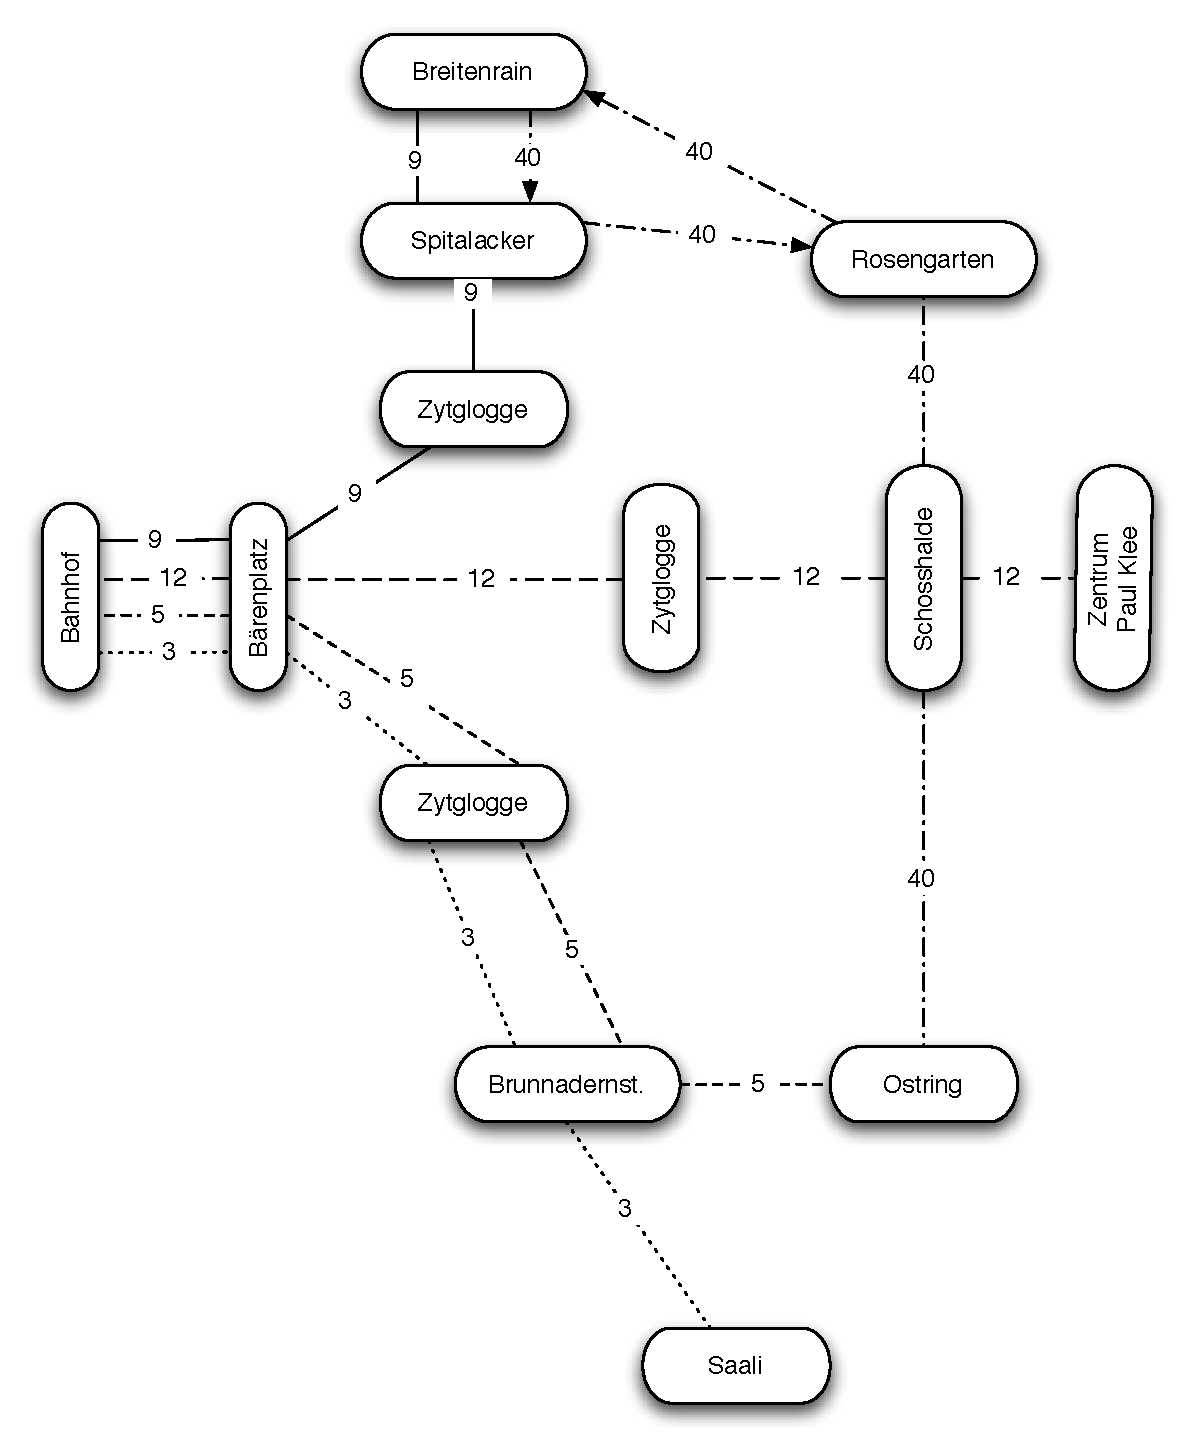
\includegraphics[width=0.6\columnwidth]{images/tram}}\caption{Simplified public transport network of Berne.}\label{tram}
\end{figure}

\noindent
The tram and bus lines shown in Fig., \ref{tram} are represented by the following database of connections:

\begin{small}
\begin{verbatim}
connected(breitenrain,spitalacker,9). 
connected(breitenrain,spitalacker,40). 
connected(spitalacker,rosengarten,40). 
connected(spitalacker,breitenrain,9). 
connected(spitalacker,zytglogge,9). 
connected(zytglogge,baerenplatz,9). 
connected(zytglogge,baerenplatz,12). 
connected(zytglogge,baerenplatz,3). 
connected(zytglogge,baerenplatz,5). 
connected(zytglogge,spitalacker,9). 
connected(zytglogge,schosshalde,12). 
connected(zytglogge,brunnadernst,3). 
connected(zytglogge,brunnadernst,5). 
connected(baerenplatz,bahnhof,3). 
connected(baerenplatz,bahnhof,5). 
connected(baerenplatz,bahnhof,9). 
connected(baerenplatz,bahnhof,12). 
connected(bahnhof,baerenplatz,3). 
connected(bahnhof,baerenplatz,5). 
connected(bahnhof,baerenplatz,9). 
connected(bahnhof,baerenplatz,12). 
connected(brunnadernst,zytglogge,3). 
connected(brunnadernst,zytglogge,5). 
connected(brunnadernst,ostring,5). 
connected(brunnadernst,saali,3). 
connected(saali,brunnadernst,3). 
connected(ostring,brunnadernst,5). 
connected(ostring,schosshalde,40). 
connected(schosshalde,zytglogge,12). 
connected(schosshalde,rosengarten,40). 
connected(schosshalde,zentrumpaulklee,12). 
connected(schosshalde,ostring,40). 
connected(zentrumpaulklee,schosshalde,12). 
connected(rosengarten,schosshalde,40). 
connected(rosengarten,breitenrain,40).
\end{verbatim}
\end{small}


\begin{enumerate}
\item Define a prolog predicate \texttt{reachable/2} which is true if you can reach the second station from the first by using one or more lines (line numbers do not matter). \textbf{( 5 points )} \vspace{5cm}
\item Define another prolog predicate \texttt{reachableBy/3} which is true if an arbitrary station is reachable from another station by a given, single line number. \textbf{( 5 points )}\vspace{5cm}
\end{enumerate}



\solution{\fontsize{8}{10}\begin{verbatim}
% b)

reachable(X,Y) :- reachableVia(X,Y,[X]). 
reachableVia(X,Y,S) :- connected(X,Y,_), not(in(Y,S)). 
reachableVia(X,Y,S) :- connected(X,A,_), not(in(A,S)), reachableVia(A,Y,[A|S]).

% c)
	
reachableBy(X,Y,Z) :- reachableByVia(X,Y,Z,[X]). 
reachableByVia(X,Y,Z,S) :- connected(X,Y,Z), not(in(Y,S)). 
reachableByVia(X,Y,Z,S) :- connected(X,A,Z), not(in(A,S)), reachableByVia(A,Y,Z,[A|S]). 

% helper
in(X,[X|_]).
in(X,[_|L]):- in(X,L).
not(X):- (X -> fail); true.
\end{verbatim}}


% - - - - - - - - - - - - - - - - - - - - - - - - - - - - - - - - - - - - - - - - - - - - - - - - - - - - - - - - - - - - - - - - - - -
\newpage
\subsection*{Points}

\begin{minipage}[t]{120pt}
\textbf{Exercise 1}
\vspace{5pt}\\
\begin{tabular}{|c|c|c|c|}
\hline
Task & Points & Score \\\hline
1 & 4 & \\\hline
2 & 4 & \\\hline
3 & 4 & \\\hline
4 & 4 & \\\hline
5 & 4 & \\\hline
\textbf{Total} & \textbf{20} &\\\hline\hline
\end{tabular}
\end{minipage}
\begin{minipage}[t]{120pt}


\textbf{Exercise 2}
\vspace{5pt}\\
\begin{tabular}{|c|c|c|c|}
\hline
Task & Points & Score \\\hline
1 & 5 & \\\hline
\textbf{Total} & \textbf{5} &\\\hline\hline
\end{tabular}
\end{minipage}
\begin{minipage}[t]{120pt}


\textbf{Exercise 3}
\vspace{5pt}\\
\begin{tabular}{|c|c|c|c|}
\hline
Task & Points & Score \\\hline
1 & 10 & \\\hline
2 & 10 & \\\hline
\textbf{Total} & \textbf{20} &\\\hline\hline
\end{tabular}
\end{minipage}
\begin{minipage}[t]{120pt}


\textbf{Exercise 4}
\vspace{5pt}\\
\begin{tabular}{|c|c|c|c|}
\hline
Task & Points & Score \\\hline
1 & 5 & \\\hline
2 & 10 & \\\hline
\textbf{Total} & \textbf{15} &\\\hline\hline
\end{tabular}
\end{minipage}

\noindent
\begin{minipage}[t]{120pt}

\vspace{1cm}

\textbf{Exercise 5}
\vspace{5pt}\\
\begin{tabular}{|c|c|c|c|}
\hline
Task & Points & Score \\\hline
1 & 2 & \\\hline
1 & 2 & \\\hline
1 & 4 & \\\hline
1 & 2 & \\\hline
\textbf{Total} & \textbf{10} &\\\hline\hline
\end{tabular}
\end{minipage}
\begin{minipage}[t]{120pt}
\vspace{1cm}

\textbf{Exercise 6}
\vspace{5pt}\\
\begin{tabular}{|c|c|c|c|}
\hline
Task & Points & Score \\\hline
1 & 5 & \\\hline
2 & 5 & \\\hline
\textbf{Total} & \textbf{10} &\\\hline\hline
\end{tabular}
\vspace{5cm}

\textbf{TOTAL}
\vspace{5pt}\\
\begin{tabular}{|c|c|c|c|}
\hline
Task & Points & Score \\\hline
1 & 20 & \\\hline
2 & 5 & \\\hline
3 & 20 & \\\hline
4 & 15 & \\\hline
10 & 10 & \\\hline
6 & 10 & \\\hline
\textbf{Total} & \textbf{80} &\\\hline\hline
\end{tabular}
\end{minipage}

\end{document}
